\subsection{Messung von Suszeptibilitäten}
Zur Bestimmund der Suszeptibilität wird die Brückenschaltung aus Abbildung
\ref{fig:schaltung} benötigt.
\begin{figure}
  \centering
  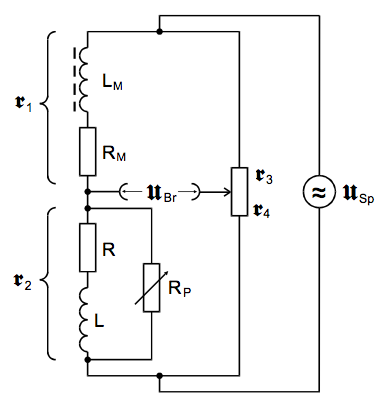
\includegraphics[width=5cm]{bilder/schaltung.png}
  \caption{Brückenschaltung zur Suszeptibilitätsbestimmung \cite{606}}
  \label{fig:schaltung}
\end{figure}
Hierbei werden zwei gleiche Spulen verwendet, da die Messung auf einer
Induktivitätsdifferenz beruht. In die eine wird das zu untersuchende
Material eingesetzt. Dabei gibt es zwei Messmethoden. Bei der einen wird die
Brückenspannung $U_\su{Br}$ gemessen, welche entsteht, wenn die Probe in eine
Spule eingeführt wird. Für Frequenzen $\omega^2L^2 >>R^2$ gilt die Vereinfachung
\begin{equation}
 \chi (\omega \to \infty) = 4 \frac{f}{Q}\frac{U_\su{Br}}{U_\su{Sp}}
\end{equation}
mit $F$ als Spulenquerschnitt, $Q$ dem Querschnitt der Probe und $U_\su{Sp}$ der
Speisespannung.
Bei der anderen Methode werden die Brücken nach dem Einführen der Probe erneut
abgeglichen. Durch die dabei auftretende Differenz an den Einstellungen
lässt sich ebenfalls die Suszeptibilität mithilfe
\begin{equation}
 \chi = 2\frac{\Delta R}{R_3}\frac{F}{Q}
\end{equation}
bestimmen. $R_3$ beschreibt den Widerstand am Potentiometer und $\Delta R$ die
Differenz der Einstellungen.
